%-------------------------------------------------
%	Version: 0.0
%	fecha de entrega
%
%-------------------------------------------------

\documentclass[11pt]{report}

%packages
\usepackage{graphicx}
\usepackage{subcaption}

\usepackage[utf8]{inputenc}
\usepackage[spanish, es-nodecimaldot]{babel}
\usepackage{setspace}
\usepackage{ragged2e}

\usepackage{amsmath}
\usepackage{amsthm}
\usepackage{amssymb}
\usepackage{mathtools}
\usepackage{siunitx}
\usepackage[thinc]{esdiff} %derivadas faciles
\usepackage{physics} %algunos simbolos de derivadas

%path donde se encuentran las imagenes
\graphicspath{ {./figuras/} }

%---------------------------------------------------------------
%ABREVIACIONES DE COMANDOS

\theoremstyle{plain}
\newtheorem{thm}{Teorema}[chapter] % reset theorem numbering for each chapter

\theoremstyle{definition}
\newtheorem{defn}[thm]{Definición} % definition numbers are dependent on theorem numbers
\newtheorem{exmp}[thm]{Ejemplo} % same for example numbers

\newcommand{\chaptercontent}{
\section{Basics}
\begin{defn}Here is a new definition.\end{defn}
\begin{thm}Here is a new theorem.\end{thm}
\begin{thm}Here is a new theorem.\end{thm}
\begin{exmp}Here is a good example.\end{exmp}
\subsection{Some tips}
\begin{defn}Here is a new definition.\end{defn}
\section{Advanced stuff}
\begin{defn}Here is a new definition.\end{defn}
\subsection{Warnings}
\begin{defn}Here is a new definition.\end{defn}
}

% REFERENCIAS
\usepackage{biblatex}
\addbibresource{ref.bib}

\begin{document}

\begin{titlepage}
\title{ADA1}

%-------------------------------------------------
%PORTADA
%-------------------------------------------------

	\centering
	{\scshape\LARGE Universidad Autónoma de Yucatán  \\ Facultad de ingeniería\par}
	\vspace{1cm}
	{\scshape\Large Instrumentación\par}
	\vspace{1.5cm}
	{\huge\bfseries Tarea 1: Simuladores de circuitos eléctricos/electrónicos\par}
	\vspace{0.7cm}
	{\begin{figure}[!h]
	\centering
    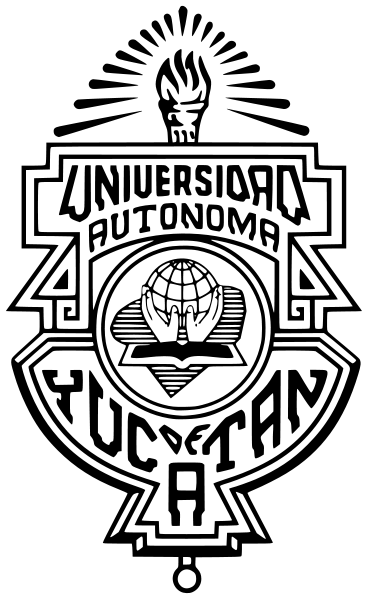
\includegraphics[scale=0.3]{UADY.png}
	\end{figure}}
	\vspace{0.7cm}
	{\Large\itshape Erick Al. Casanova Cortés\par}
	{\Large\itshape Matricula: 15014866\par}
	\vfill
	{\scshape\Large Docente\par
	Dr. Renan Quijano\par}
	\vfill
	{\Large{\bfseries Fecha de entrega: 2 Marzo 2021} }

	\vfill
	
\end{titlepage}

%-------------------------------------------------
%Inicio del documento
%-------------------------------------------------

\tableofcontents

%-------------------------------------------------
% Instrucciones
%-------------------------------------------------

\chapter{Instrucciones}


%-------------------------------------------------
% Planteamiento

\section{Planteamiento}

Los simuladores de circuitos eléctricos y electrónicos, son una herramienta útil para analizar y predecir el comportamiento de los circuitos ante diferentes condiciones de entrada o diferentes configuraciones de los componentes.

Existe un gran número de simuladores de uso libre y es importante aprender a utilizarlos antes de implementar un circuito en el laboratorio.


%-------------------------------------------------
% Desarrollo

\section{Desarrollo}

Para realizar la tarea debe seguir los siguientes pasos:

\begin{enumerate}
	\item Investigar en internet acerca de los simuladores de circuitos electrónicos gratuitos disponibles.
	\item Seleccionar tres opciones de simuladores que le parezcan atractivos e indicar las características que los hacen atractivos.
	\item Incluir enlace para acceder a los simuladores.
	\item Integrar la información recabada en un reporte en formato pdf.
	\item Subir el archivo a la plataforma UADY virtual, en el espacio correspondiente para el envío de Tarea1: Simuladores de circuitos eléctricos/electrónicos.
\end{enumerate}


%-------------------------------------------------
% Simuladores
%-------------------------------------------------

\chapter{Simuladores gratuitos}

Debido a la pandemia muchos cursos escolares dentro de la facultad de ingeniería se han visto frustrados por la falta de prácticas de laboratorio que se puedan realizar fuera de la misma facultad, por lo mismo la simulación de distintos fenómenos o el análisis computacional es una opción viable para contrarrestar las dificultades que la actualidad nos presenta.


Para la materia de Instrumentación los laboratorios son parte esencial para el alumno, ya que ahí es donde se entablan los conocimientos de la materia. Por lo mismo es menester conocer las herramientas que podemos utilizar.


A continuación se presentarán tres simuladores de circuito online que son gratuitos o accesibles a un estudiante de la Universidad Autónoma de Yucatán.


%-------------------------------------------------
% Falstad

\section{Falstad}

Falstad es una herramienta web que no requiere ni una cuenta para utilizar, puede simular gran cantidad de componentes electrónicos. Incluso cuenta con una versión offline que requiere de instalación llamado \textit{Standalone} el cual puede ser instalado en los sistemas operativos Linux, MacOs y Windows.\\


\begin{figure}[!h] %Captura Falstad
	\centering
	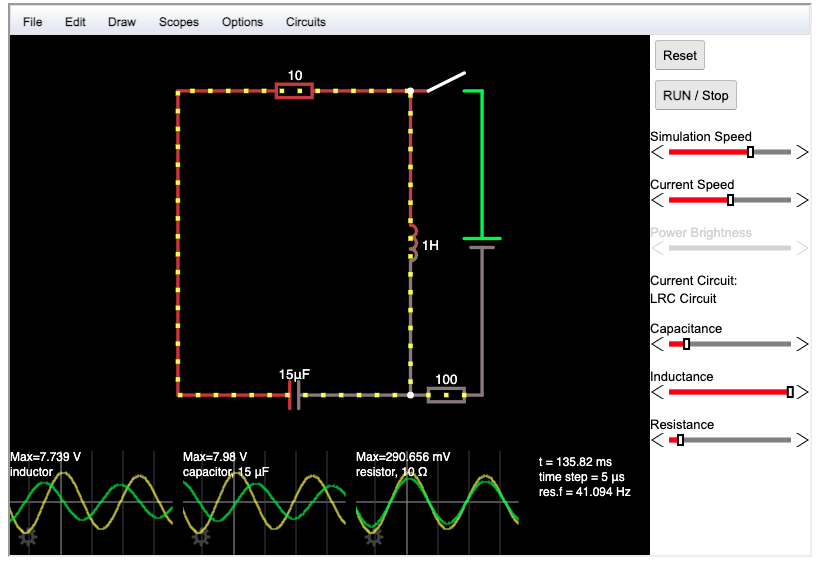
\includegraphics[scale=0.3]{Falstad.png}
	\caption{Captura del la interfaz de Falstad}
	\label{fig:Falstad}
\end{figure}



En sí es una herramienta bastante útil porque puede generarnos gráficas como si fuera un osciloscopio, podemos ver en la figura \ref{fig:Falstad} como se presenta al usuario con un ejemplo de su funcionamiento.\\
Se puede notar que posee herramientas ya predeterminadas y un manual dentro de la misma página web.


Este se puede acceder en la siguiente página \url{https://www.falstad.com/circuit/index.html}\\

La parte negativa de este programa es que no posee microcontroladores 

%-------------------------------------------------
% Tinkercad

\section{Tinkercad}

Tinkercad es otro simulador bastante amigable con el usuario, a diferencia del anterior, la manera de diseñar circuitos es a travez de un protoboard y se van arrastrando los componentes como si se estuviesen conectando de manera física.\\

\begin{figure}[!h] %Captura Tinkercad
	\centering
	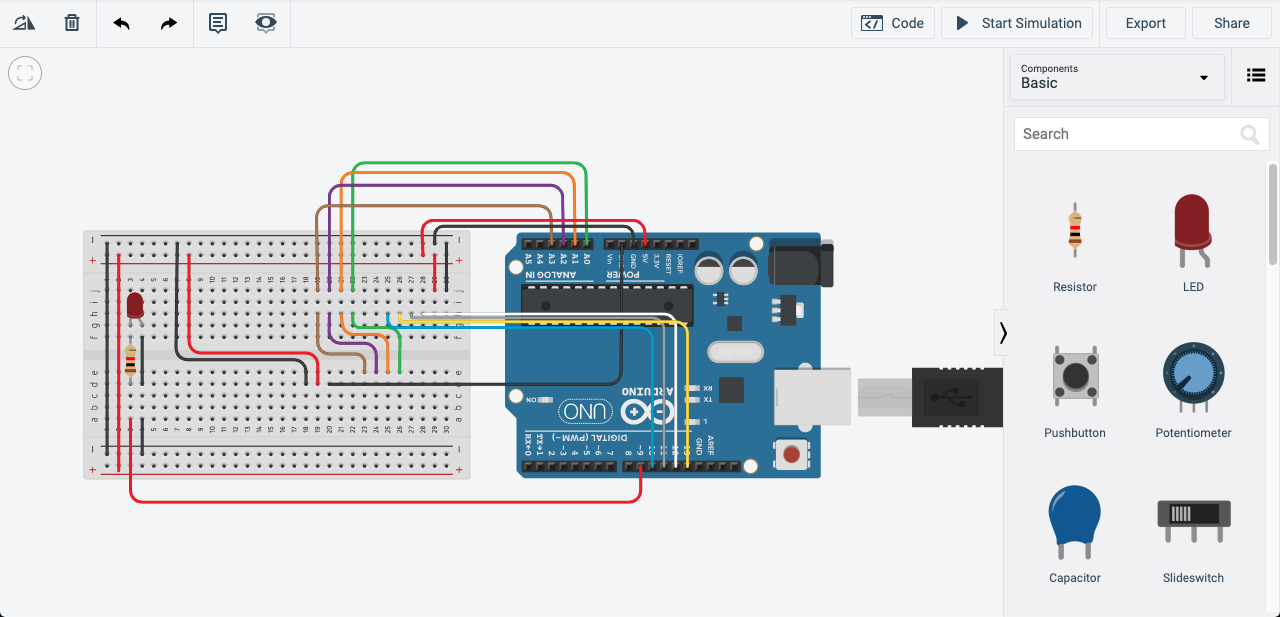
\includegraphics[scale=0.3]{Tinkercad.png}
	\caption{Captura del la interfaz de Tinkercad}
	\label{fig:Tinkercad}
\end{figure}

Para acceder a este se requiere tener una cuenta CAD, la cual debe ser creada con el correo institucional ya que la universidad cuenta con el servicio.\\

Una vez con la cuenta CAD podemos hacer total uso de las herramientas que no brinda, en sí el programa es bastante auto-explicativo y cuenta con un apartado en la nube donde se pueden guardar los circuitos en los que hemos trabajado.\\
También cuenta con distintos Arduinos, por lo que podría ser de bastante ayuda cuando se trate de hacer los ejercicios, prácticas o proyectos de la materia.\\

Se puede acceder con la siguiente liga: \url{https://www.tinkercad.com/}


%-------------------------------------------------
% Multisim

\section{Multisim}


Por último pero no menos importante está el Multisim, este programa cuenta con una versión gratuita, aunque para acceder a esta necesitamos crear una cuenta, la cual no tiene costo.\\
Podría verse como una versión más completa que el Falstad, ya que cuenta al igual que Tinkercad con una nube donde uno puede almacenar los circuitos en los que ha trabajado, también cuenta con múltiples componentes electrónicos aunque también carece de microcontroladores, así como privacidad, ya que todos los circuitos que guardemos en su nube serán de carácter público. Otro problema es el espacio de trabajo, al usar la cuenta gratuita solo nos permite un espacio de trabajo reducido en el cual se pondrá el circuito, lo cual puede llegar a frustrar el trabajo

El enlace para utilizar dicho programa es: \url{https://www.multisim.com/}

 
\begin{figure}[!h] %Captura Multisim
	\centering
	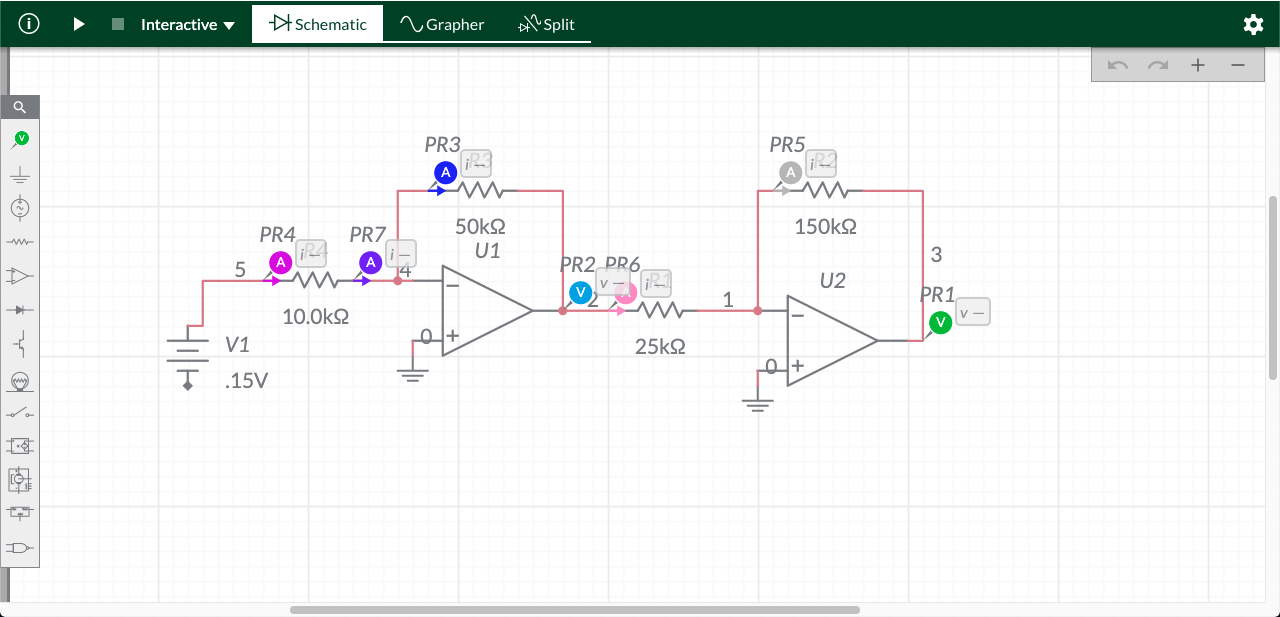
\includegraphics[scale=0.3]{Multisim.png}
	\caption{Captura del la interfaz de Multisim}
	\label{fig:Multisim}
\end{figure}

%-------------------------------------------------
%Referencias
%-------------------------------------------------

\nocite{noauthor_circuit_nodate}
\nocite{noauthor_dashboard_nodate}
\nocite{noauthor_multisim_nodate}

\printbibliography


%-------------------------------------------------
%Final del documento
%-------------------------------------------------
\end{document}
